\documentclass[journal=jpclcd,manuscript=article]{achemso}
\pdfoutput=1
\usepackage{gensymb}
\usepackage{amsmath}
\usepackage{graphicx}
\usepackage{epsfig}
\usepackage{multirow}
\usepackage{multicol}
\usepackage{color}

\author{Jason Codrington$^{\dagger}$}
\affiliation{Department of Chemistry, William Paterson University, 300 Pompton Road, Wayne, NJ, 07470, USA}
\author{Noor Eldabagh$^{\dagger}$}
\affiliation{Department of Chemistry, William Paterson University, 300 Pompton Road, Wayne, NJ, 07470, USA}
\author{Kimberly Fernando$^{\dagger}$}
\affiliation{Department of Chemistry, William Paterson University, 300 Pompton Road, Wayne, NJ, 07470, USA}
\author{Jonathan J. Foley IV}
\affiliation{Department of Chemistry, William Paterson University, 300 Pompton Road, Wayne, NJ, 07470, USA}
\email{foleyj10@wpunj.edu}

%Title of paper
\title{Unique hot carrier distributions from scattering mediated absorption}
% Date
\date{\today}


% Being document
\begin{document}

\begin{tocentry}
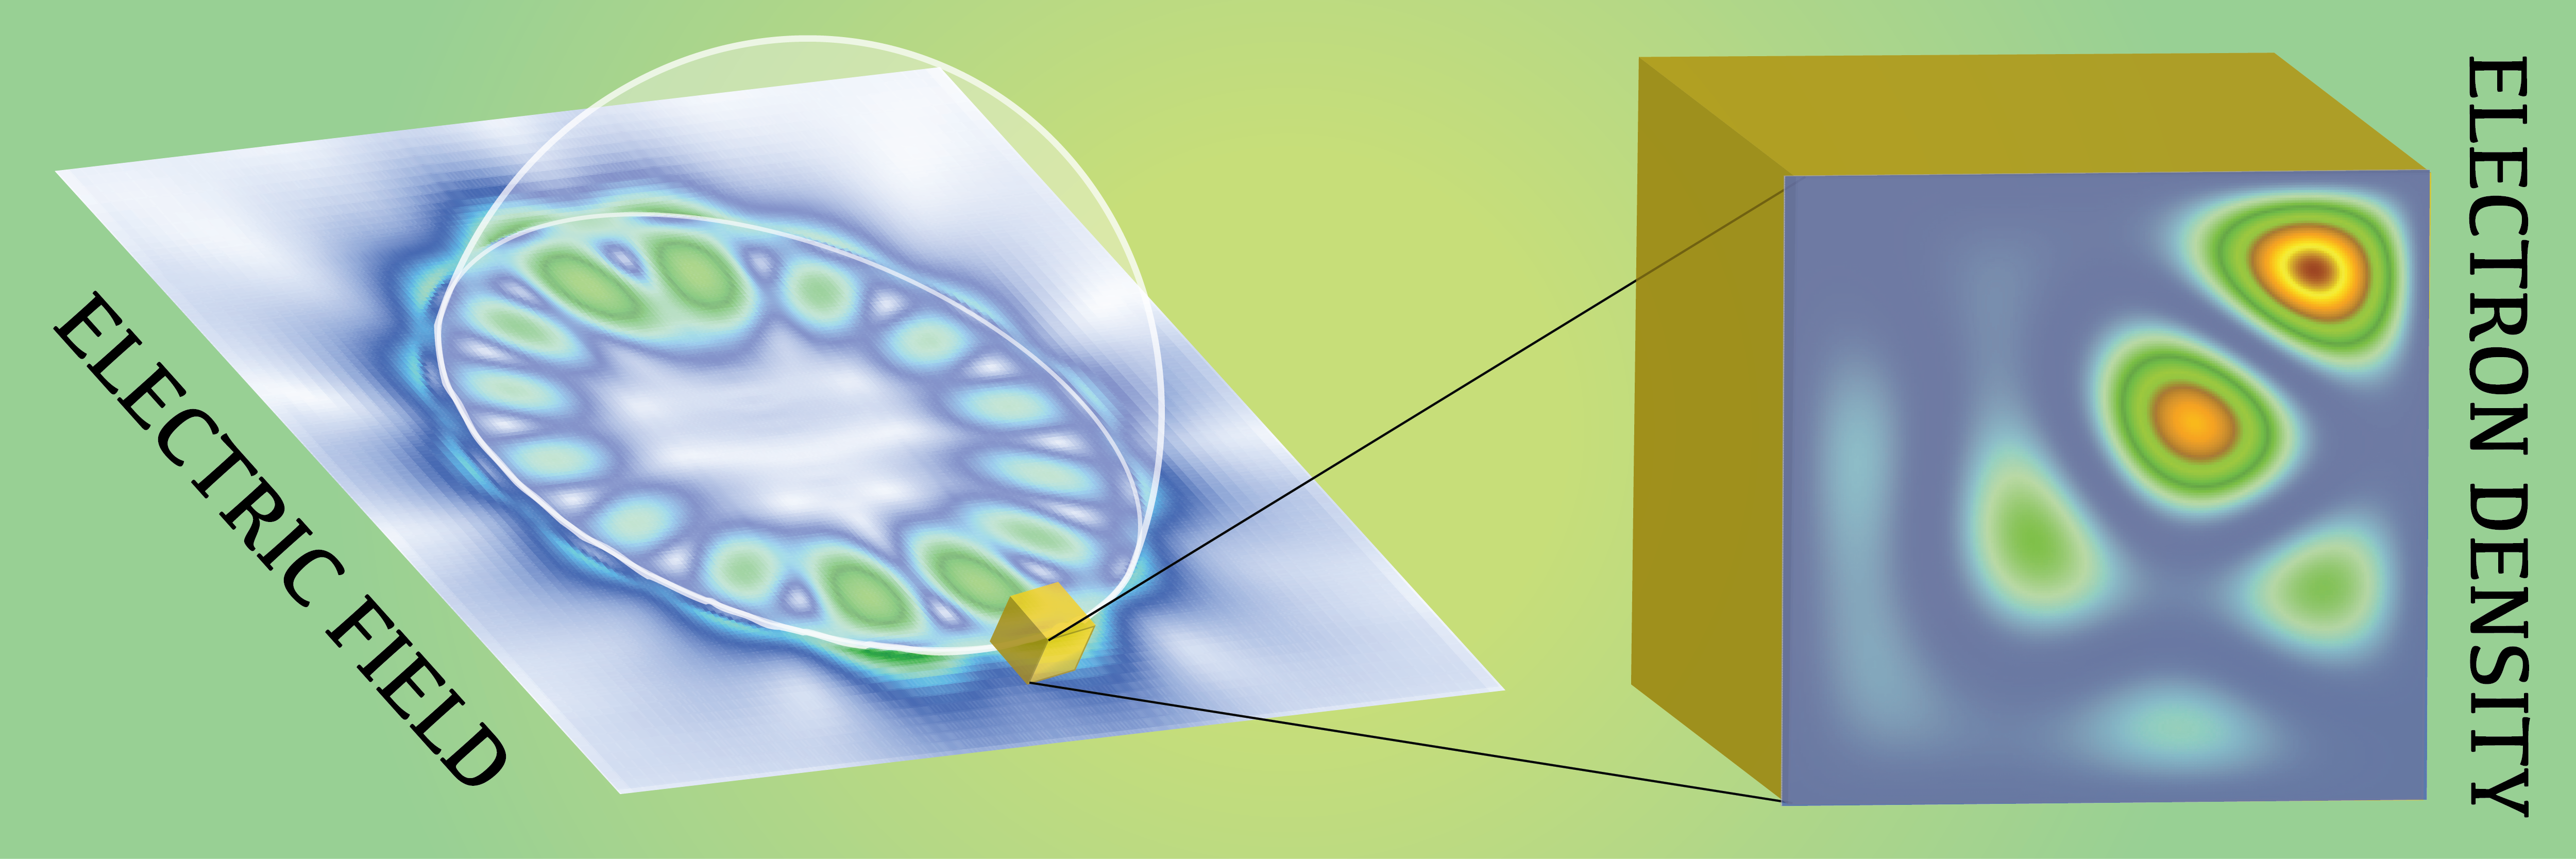
\includegraphics[width=9cm]{nanosphere_WGMv3.png}
\end{tocentry}

\begin{abstract}

Light-initiated generation of energetic carriers has attracted considerable attention as a paradigm for 
photocatalysis and solar energy conversion, and the use of noble metal nanoparticles that support localized surface
plasmon resonances has been widely explored as a medium for realizing this paradigm.  It was recently
shown that composite nanostructures enable the interplay between dielectric scattering resonances and broad-band
absorption in small metal nanostructures, a phenomenon termed scattering mediated absorption, can be 
used to mediate energetic carrier transfer and selective photochemistry with 
low-intensity light while completely circumventing plasmon resonance.  In this work, we develop 
a multi-scale modeling approach for elucidating the hot carrier dynamics initiated by scattering mediated
absorption.  Our calculations reveal that unique hot carrier distributions and dynamics arise 
from scattering mediated absorption as compared to plasmon excitation, and also suggest that in 
a variety of circumstances, scattering mediated absorption may lead to more
efficient hot carrier generation compared to plasmon resonance under the same external illumination
conditions.  These results are an important first step in understanding the phenomena of
scattering mediated hot carrier generation, which has potential for expanding the
palette of materials that can be utilized for hot carrier mediated photochemistry beyond plasmonic metals,
and for enabling unique pathways for photocatalytic transformations.
\end{abstract}

%%\maketitle

%%\end{document}

%%\section{Introduction}

Various strategies that exploit the optical properties of metal nanoparticles, namely their ability to support localized surface plasmons resonances [LSPR], 
which are collective oscillations of their 
conduction electrons driven by light, have been explored recently with the aim of using low-intensity light to efficiently drive chemical 
reactions~\cite{LCI_NatureMater_2011,KAC_ACSCatalysis_2013,ZLQ_RSCAdvances_2015,PKL_AccChemRes_2015}.  The interest in this area has 
been motivated partly by the fact that metal nanoparticles (most prominently silver and gold) are exceptionally good absorbers of visible light; therefore,
they are ideal candidates for harvesting solar photons~\cite{AP_NatMat_2010}.  
Importantly, the resonant properties of plasmonic particles are highly tunable by parameters under synthetic control such as geometry, composition, surface chemistry, and the surrounding 
environment~\cite{SX_Science_2002,BCN_ChemRev_2005,GB_NatPhoton_2010}.  An emerging paradigm that exploits LSPR for photocatalysis is known as Plasmon-mediated Hot-Electron Transfer [PHET],
and a growing number of reports are demonstrating the ability of PHET to catalyze energetically demanding chemical 
reactions~\cite{CXL_NatureChem_2011,MZL_Science_2013,MLL_NanoLett_2013,LFP_AC_2015,ZHX_NatPhoton_2016,ZJM_ACSNano_2016,SZZ_PNAS_2016,SCR_JPCC_2016}.

In PHET, the collective plasmon excitation decays rapidly (on a ~10 femtosecond timescale) to a non-equilibrium distribution of energetic electron-hole pairs, or a so-called hot carrier 
distribution~\cite{KAC_ACSCatalysis_2013,GZG_JPCC_2013,SNJ_NatComm_2014,WCM_Science_2015,MWW_NatComm_2015, BSN_ACSNano_2016}.  
Hot carriers can deposit energy into reactive degrees of freedom of molecules adsorbed 
to the nanoparticle surface, thereby initiating chemical transformations.  Despite 
the considerable progress made in 
demonstrating the potential of PHET, its widespread application 
faces several challenges. The intrinsic optical properties of noble metals that 
give rise to the extraordinarily 
large absorption cross sections associated with LSPR are also fundamentally 
related to the broad energy spectra and short lifetimes associated with LSPR 
and the subsequent hot carrier 
distributions~\cite{KS_JCP_1983}. 
Furthermore, the timescale of hot carrier relaxation competes 
with transfer to adsorbate states (both occur on 100 fs timescales), which fundamentally limits the efficiency of energy transfer~\cite{WCM_Science_2015}.  \textcolor{red}{Finally, there are a limited number of materials that show promising plasmonic
behaviors (most prominently silver and gold), and it is desirable to extend the palette of available materials to include
non-precious metals and metals with broader applicability in catalysis~\cite{SZZ_PNAS_2016}.}

Considering this, an incredible opportunity exists to identify new classes
of materials capable of mediating light-matter interactions and energy transfer events that offer the same advantages as metal nanoparticles, 
namely exceptional light-harvesting potential, while also offering greater selectivity and efficiency in energy transfer, as well as tunable surface chemistry for enhanced catalytic activity.  
Ideally, such structures could be made mostly, if not entirely, from cost-effective materials.  Recent progress towards this aim has been made by designing hybrid 
nanostructures that effectively delegate the light-harvesting and catalytic functions to separate components of the structure.  Recently, Halas and co-workers 
demonstrated an antenna-reactor concept that leverages the near-field enhancement from aluminum plasmons to generate energetic carriers on 
palladium islands and showed the efficacy of this strategy for the photcatalytic transformation of acetylene to ethylene~\cite{SZZ_PNAS_2016}.
Two of the current authors, along with Sun and co-workers, demonstrated a phenomena known as scattering mediated absorption [SMA] where dielectric
scattering resonances in SiO$_2$ nanospheres were utilized to induce resonant absorption in non-plasmonic platinum nanoparticles in SiO$_2$/Pt nanohybrids~\cite{ZHX_NatPhoton_2016}.
The SMA phenomena was also observed to induce highly selective photocatalytic oxidation of benzyl alcohol to benzaldehyde~\cite{ZHX_NatPhoton_2016}.
Zhang {\it et al.} independently described a SMA phenomenon in Au-TiO$_2$ nanohybrids that leveraged so-called whispering gallery modes to 
enhance plasmonic and non-plasmonic absorption in gold nanoparticles, and demonstrated these structure's efficacy for photocatalytic water splitting~\cite{ZJM_ACSNano_2016}.
Interestingly, hot carrier transfer was implicated in the photocatalytic mechanisms that resulted from these SMA phenomena~\cite{ZHX_NatPhoton_2016,ZJM_ACSNano_2016}.
The prospect of using SMA in hybrid dielectric/metal nanostructures to initiate hot carrier generation and transfer is particularly 
compelling as it could completely circumvent plasmon excitation.  Not only does this open up possibilities to utilize a broad palette of earth-abundant and cost-effective materials, it also
presents the possibility of realizing unique photocatalytic pathways owing to differences in the distributions and dynamics of energetic carriers produced by SMA compared
to those produced by plasmon excitation.    

The push to identify novel structures for mediating hot carrier generation and transfer has been paralleled by 
efforts to develop theoretical methodologies to elucidate these processes.  The underlying electronic
structure has been treated both within free-electron models confined by potential wells~\cite{GZG_JPCC_2013,ZG_JPCC_2014,MLK_ACSNano_2014,KPB_SciRep_2015,SAG_ACSPhotonics_2016} (here called
``particle-in-a-well" [PIW] models), as well as by {\it ab initio} approaches~\cite{SNJ_NatComm_2014,BMN_NatComm_2015,MWW_NatComm_2015,BSN_ACSNano_2016}.
Using PIW models, Govorov and co-workers developed a theory of 
hot carrier generation within the framework of time-dependent perturbation theory that
has elucidated a variety of shape- and size-dependent factors for optimizing 
the hot carrier generation~\cite{GZG_JPCC_2013,ZG_JPCC_2014}.  A similar approach was also pursued by Kumarasinghe {\it et al.} suggesting
that nanorods are exceptionally good structures for hot carrier generation~\cite{KPB_SciRep_2015}.  Garc\'ia de Abajo and co-workers recently described a 
quantum master equation approach with an underlying PIW model that elucidated a number of key factors that influence
hot carrier excitation and decay dynamics~\cite{SAG_ACSPhotonics_2016}.  The utilization of {\it ab initio} approaches by Sundararaman {\it et al} 
has also provided valuable insights into the role that a metal's band-structure plays
in determining the efficiency of hot carrier generation, and particularly in the asymmetry between hot-electron
and hot-hole generation~\cite{SNJ_NatComm_2014}.  Nordlander and co-workers have directly compared free-electron and {\it ab initio} approaches
and found negligible impact on hot carrier generation and dynamics in Ag nanospheres resulting from electron correlation~\cite{MLK_ACSNano_2014}.  \textcolor{red}{However, many-body effects are not negligible for hot-carrier dynamics
in general; for example, Bernardi {\it et al} have demonstrated that many-body effects are important 
in the overall hot carrier dynamics resulting
from surface plasmon polaritons in gold, and also in the decay mechanisms for hot-carriers in silver~\cite{BMN_NatComm_2015}.}

We develop a novel approach for studying hot carrier dynamics that may arise from arbitrary electromagnetic
fields, including the unique near-fields that arise from SMA on hybrid dielectric-metal nanoparticles and LSPR
on noble metal nanoparticles.  Importantly, this method goes beyond a perturbative inclusion of the electric field and enables us to follow the electronic degrees of freedom subject to strong fields with arbitrary time-dependence, which are characteristic of SMA and LSPR.   

We consider the electronic degrees of freedom on the metal nanoparticle subject to the time-dependent Hamiltonian 
\begin{equation}\label{eq:TDHam}
\hat{H}(t) = \hat{H}_{el} - {\bf E}(t) \cdot \hat{\mu}, 
\end{equation}
where the specific form of ${\bf E}(t)$ derives from a rigorous time-domain electrodynamics calculation with a realistic model
of the nanostructures in question and $\hat{H}_{el}$ describes non-interacting electrons confined to metal nanocubes [NCs] by an infinite potential well.  
We compute the time-domain field 
using a commercial simulator based on the finite-difference time-domain [FDTD] method~\cite{Lumerical}.  
Incorporating  ${\bf E}(t)$ from these FDTD simulations into the time-dependent Hamiltonian enables us to investigate the unique ways
in which the electronic degrees of freedom evolve under the influence of the distinct time-varying fields that result
from LSPR and from dielectric scattering resonances, allowing us a unique window into the hot carrier dynamics resulting from LSPR as compared
to SMA.  Further details on the FDTD simulations can be found in the Supplementary Information [SI]. 

The many-electron wavefunction of the metal nanoparticles is expanded in terms of a configuration-interaction expansion that
includes all singly-excited configurations~\cite{Szabo},
\begin{equation}\label{eq:CIS}
|\Psi_{CIS}\rangle = c_0 |\Phi_0 \rangle + \sum_{i,a} c_i^a |\Phi_i^a\rangle,
\end{equation}
where the configuration $|\Phi_i^a\rangle$ has an electron excited from orbital $i$ to orbital $a$, 
and $c_0$ and $c_i^a$ are complex expansion coefficients.  Unless otherwise specified, indices $i, j$ will indicate
orbitals which are occupied in the ground state reference configuration and indices $a, b$ will indicate orbitals
which are unoccupied in the ground state reference.  

The time-evolution of the wavefunction can be subsumed in the expansion coefficients, which allows the TDSE to be written 
\begin{equation}\label{TDCIS}
i\hbar \frac{ d}{dt} {\bf c}(t) = {\bf H}(t) {\bf c}(t)
\end{equation}
where ${\bf c}(t)$ is the vector of complex expansion coefficients and ${\bf H}(t)$ is the time-dependent Hamiltonian
matrix.  The Hamiltonian matrix is comprised of three unique classes of elements in the CIS model,  
\begin{equation}
  {\bf H}(t) 
  \mbox{=}
  \begin{pmatrix}
    \langle \Phi_0 | \hat{H}(t) | \Phi_0 \rangle    &     \langle \Phi_0 | \hat{H}(t) | \Phi_i^a \rangle    \\
  \langle \Phi_j^b | \hat{H}(t) | \Phi_0 \rangle    &   \langle \Phi_j^b | \hat{H}(t) | \Phi_i^a \rangle \end{pmatrix}.
\end{equation}
Explicit expressions for each class of matrix elements are given in the SI.
\textcolor{red}{Importantly, the lower diagonal block of the CIS Hamiltonian matrix contains terms which couple together
different excited configurations.  In particular, transitions between singly-excited configurations which differ
in only one unoccupied index ($|\Phi_i^a\rangle \rightarrow |\Phi_i^b\rangle$) or which differ in only one occupied index
 ($|\Phi_i^a\rangle \rightarrow |\Phi_j^a\rangle$) are enabled by the terms in the lower diagonal block.  Such excited-state to excited-state transitions are absent from approaches based including linear response TDDFT and approaches which use time-dependent perturbation
 theory to first order, as these only include transitions between ground- and singly-excited configurations ($|\Phi_0\rangle \rightarrow |\Phi_i^b\rangle$)%%%%% Need citations here!.
The ($|\Phi_i^a\rangle \rightarrow |\Phi_i^b\rangle$) and ($|\Phi_i^a\rangle \rightarrow |\Phi_j^a\rangle$) are important in this context because the fields that arise from SMA continue to evolve on long ($>$100 fs) timescale.  On this timescale, population can 
accumulate in excited-state configurations, enabling the SMA fields to drive transitions between excited configurations as well as from the 
ground-state configuration (see Supporting Information and Figure S4 for more details).} 

Given the simplicity of the underlying electronic Hamiltonian, the field-free Hamiltonian matrix is diagonal, and only the dipolar
interaction of the nanoparticle with the external field can induce transitions among the electronic configurations, hence the treatment in 
this work neglects excited-state thermalization contributions from electron-electron scattering.  
\textcolor{red}{As shown in previous work, the inclusion of many-body effects can impact the calculation
of hot-carrier distributions when transitions from $d$ bands are relevant, which is in principle whenever the perturbing
field contains frequency components that overlap with interband transitions involving $d$ bands~\cite{MLK_ACSNano_2014,BMN_NatComm_2015, Atwater_Review}.  
In this work, we explore SMA involving Ag and Pt nanoparticles, and we wish to emphasize that the many-body effects 
which are neglected in this work are expected to have an impact on the hot-carrier distributions in both of these metals, 
as both have energetic gaps between the $d$-band and the Fermi level which are smaller than energy components of the optical fields
considered here.  Examination of these two metals within our model still presents considerable value because it provides
insight into hot-carrier dynamics in two distinct regimes of the driving field, which includes a superposition
of the plasmon and dielectric scattering fields.  In particular, these regimes include (1) when the plasmon 
resonance and the dielectric scattering resonance overlap in energy with transitions in the quantum model 
(i.e. SMA involving Au, see Figure 1 (d)), 
and (2) when only the dielectric scattering resonances overlap with 
quantum transitions (i.e. SMA involving Pt, see Figure 2 (d)).   
We also choose Au and Pt because the SMA phenomenon
has been experimentally demonstrated in both metals, including in the work by Sun and co-workers~\cite{ZHX_NatPhoton_2016} which
considered SiO$_2$ nanospheres decorated with Pt nanoparticles of similar size to the particles considered here, and the work of 
Zhang {\it et al.}~\cite{ZJM_ACSNano_2016} which considered
TiO$_2$ nanospheres decorated with large Au nanoparticles.  It has been shown that many-body effects have less of an impact
on hot-carrier dynamics in Ag nanoparticles due to the relatively large ($> 3eV)$ gap between the $d$ bands and the Fermi level~\cite{MLK_ACSNano_2014,Atwater_Review}, and so
analogous calculations have been performed on Ag-decorated nanospheres showing similar qualitative features
as results with Au and Pt (see Supporting Information and Figure S3).
  Future work will focus on further developments of this modeling approach to include
many-body effects, and investigation of these effects on the hot-carrier distributions and dynamics resulting from SMA.  It is expected
that these effects will play a role in the hot-carrier dynamics in several ways, including by changing the available excitation/transition channels
by mixing of the single-particle states, modifying the transition rates through modification of transition dipole moments, and by enabling
thermalization of the excited carriers through electron-electron scattering.}

Because of the diagonal nature of the field-free Hamiltonian, each configuration $|\Phi_i^a\rangle$ is an eigenfunction
of the field-free Hamiltonian.  This simplifies the interpretation of the electronic structure relative to the CIS 
wavefunction in quantum chemistry applications where electron repulsion is included in the Hamiltonian
and the excited electronic eigenfunctions are linear combinations of singly-excited configurations. 
The multiplication of the Hamiltonian matrix on the coefficient vector generates the gradient of the coefficient vector in time, and
a variety of algorithms have been developed to use this information to propagate the wavefunction in time.  Here we use a symplectic integrator
described in Ref.~\citenum{SP_JCP_96}.  Propagation of the CIS wavefunction is referred to as the TDCIS method 
throughout~\cite{KKS_JCP_2005,GHP_PRA_2010,DPG_PRL_2011}.

We analyze the hot carrier distribution and dynamics that results from SMA and LSPR excitation by computing the 
instantaneous populations of orbitals both above and below the Fermi level of the metal nanostructure.   
In our model, the orbitals are energy eigenstates of a 1-electron Hamiltonian and have well-defined kinetic energy,
and the orbital populations are given by the diagonal elements of the 1-electron reduced density matrix [1-RDM],
\begin{equation}
^1D^q_q(t) = \langle \Psi(t) | \hat{a}^{\dagger}_q \hat{a}_q | \Psi(t) \rangle,
\end{equation} 
where the second-quantized operator $\hat{a}_q^{\dagger}$ ($\hat{a}_q$) creates (kills) an electron
in orbital $q$~\cite{Szabo}.  \textcolor{red}{The hot-carrier populations plotted in Figures 1 and 2 panels (e) and (f)
are computed as $^1D^q_q(t)-^1D^q_q(t=0)$, and similarly for the change in occupations plotted
in Figure 3 panels (b) and (c).} The orbital indices can be uniquely mapped to the relevant orbital quantum numbers ($n_x, n_y, n_z$ for
the PIW NC model) so that the orbital energies can be readily computed (see SI for more details). 

\begin{figure}
\begin{center}
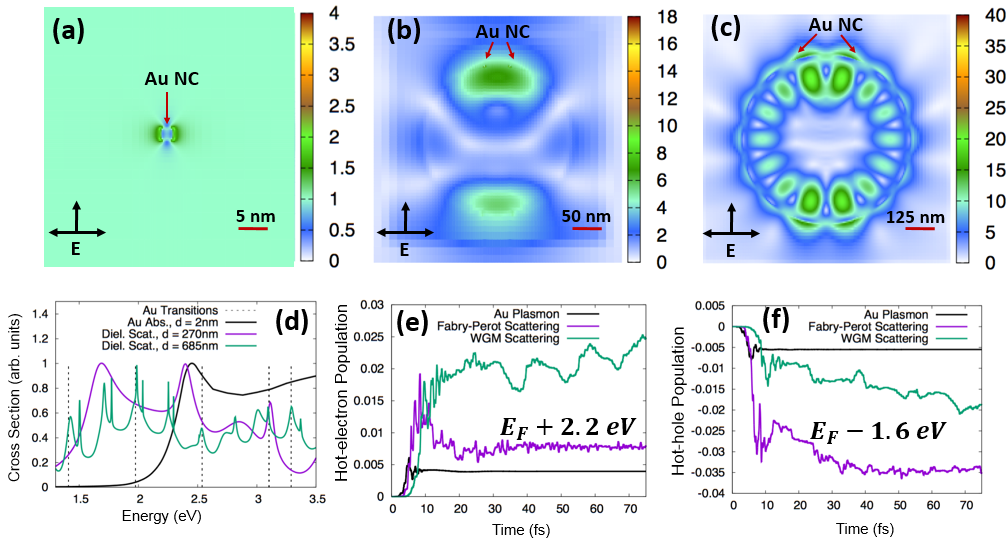
\includegraphics[width=6in]{Au_AllThree_Revision.png}
\caption{Three regimes for light-matter interactions leading to unique
spatial and temporal shaping of the incident field, and the corresponding
impact on electronic dynamics in a $L=2nm$ PIW Au nanocube. Plots of the near-field enhancements (${\bf |E|}/{\bf |E_0|}$) are shown for the
Au NC LSPR ($\lambda=532 nm$, {\bf Panel (a)}), a Fabry-Perot resonance of a d=270nm dielectric nanosphere decorated with Au NCs ($\lambda = 397 nm$, {\bf Panel (b)}),
and a Whispering Gallery Mode resonance of a d=685 nm dielectric nanosphere decorated with Au NCs ($\lambda = 493 nm$, {\bf Panel (c)}).
The extinction spectra of these three structures are shown overlaid with the dipole-allowed transitions in the PIW model of the Au NC, showing particularly
strong overlap between these transitions and the scattering resonances of the $d=685 nm$ dielectric nanosphere ({\bf Panel (d)}).
The hot-carrier populations ($^1D_p^p(t)-^1D_p^p(t=0)$) are computed to measure hot-electron and hot-hole generation.
Both dielectric scattering resonances show more efficient generation of hot-electrons ({\bf Panel (e)}) and hot-holes ({\bf Panel(f)}) compared to LSPR in this case.}
\end{center}
\end{figure}

%% E_f gold is 5.52 eV, Nels = 472
%% E_f Pt   is 9.40 eV, Nels = 1104
The TDCIS approach is applied to investigate hot carrier dynamics of $L=2nm$ gold and platinum NCs that are (a) free-standing so that
the dynamics are induced by optical resonances supported by the NC alone and (b) supported on various dielectric nanospheres so
that the dynamics are also induced by time-evolving nearfields arising from dielectric scattering resonance.  We choose these metals because 
attachment of gold and platinum metal nanoparticles to various sized dielectric nanospheres has been experimentally demonstrated; future
work will investigate similar phenomena with non-precious metals.
The electronic structure
of these model NCs are distinguishable by their Fermi energies and the number of electrons: the Au NC model has a Fermi energy
of 5.52 eV (compared to the bulk value of 5.53 eV) and 472 electrons, the Pt NC model has a Fermi energy of 9.40 eV (compared to the bulk
value of 9.75 eV) and 1104 electrons. 
In this work, 4900 singly-excited configurations are included in $|\Psi_{CIS}\rangle$ for both Au and Pt NCs.  
Despite the large number of excited states included in our many-electron wavefunctions, the high 
degeneracy of the underlying dipole-allowed transitions leads to a relatively small number of visible spectroscopic lines for the Au (see Figure 1 (d))
and Pt models (see Figure 2 (d)). 

The spectral flexibility of dielectric scattering
resonances allows tuning to overlap with one or more of these transition energies via the nanosphere size; in contrast, for very small 
metal nanoparticles, the position of the LSPR is intrinsically related to the relative permittivity of the metal~\cite{Bohren}.  This is
illustrated by plotting the scattering spectrum of a moderate-sized ($d=270nm$) and large ($d=685nm$) dielectric nanospheres and the 
absorption spectrum of a small ($d=2nm$) gold nanosphere all computed via Mie theory~\cite{Bohren}.  These Mie spectra are overlaid with the dipole-allowed
transitions in our PIW model of the Au NC (see Figure 1(d)). The $d=270nm$ dielectric nanosphere has a relatively broad scattering resonance 
(herein referred to as a Fabry-Perot [FP] resonance) that overlaps 
with a PIW Au NC transition at 3.1 eV, and
a $d=685nm$ dielectric nanosphere has narrow scattering resonances (whispering gallery modes [WGM]) 
that overlap with multiple transitions between 1.3 and 3.3 eV.  The $2nm$ Au nanosphere has a broad absorption peak associated with its LSPR that partially
overlaps with a dipole-allowed transition in the PIW Au NC at 2.5 eV. 

As proxies of the hot carrier dynamics in the Au NC, we plot the population dynamics of the highest and lowest energy orbitals in the Au NC active space, which lie
2.2 eV above and 1.6 eV below the Fermi energy, respectively (Figure 1 (e) and (f)).  Snapshots of the populations of all active
orbitals in the Au NC model at various times are also provided in the SI (see Figure S1).  
We observe that the LSPR generates a relatively small
population of hot carriers with field-driven dynamics that evolve on a short (~10 fs) timescale.  FP resonance in this
case leads to significantly more efficient hot-hole generation with field driven dynamics that evolve on a moderate (~50 fs) timescale (Figure 1(f)), while
WGM resonances lead to considerably more efficient hot-electron generation with field drive dynamics that evolve on a much longer (~200 fs) timescale
(Figure 1(e) and Figure 3(b)).  Another key distinction between the hot carrier density generated by the Au LSPR and by SMA is that the hot-carrier density
of the former is concentrated within 1 eV of the Fermi level, while SMA leads to appreciable density $\pm 2$ eV of the Fermi level (see Figure S1).

These differences can be attributed in part to the unique ways in which each resonant interaction simultaneously modulates the incident optical
fields in space and in time. An illustration of spatial confinement associated with each resonance can be seen in the
electric field intensity maps at the resonance frequency for the
Au LSPR (Figure 1(a)), FP resonance (Figure 1(b)), and WGM resonance (Figure 1(c)); all resonances lead to approximately 1 order of
magnitude nearfield enhancement in the vicinity of the Au NC.
A progression of resonance lifetimes can be inferred from the extinction spectra of the Au LSPR, the FP resonance, and the WGM resonance, with
the Au LSPR having the broadest extinction peak and the shortest lifetime, and the WGM having the most narrow extinction peaks and longest lifetimes.  These
lifetimes determine the period of time that the metal electrons are being driven by enhanced nearfields associated with the optical resonances, and
the long lifetime associated with the WGM means that the nearfield that drives the metal electrons continues to evolve on a relatively long timescale compared
to the electronic dynamics.
Longevity of the evolution of the electric field resulting from dielectric scattering resonances is consistent with the 
longer period of population transfer from the Fermi level and below to higher unoccupied orbitals when compared with surface plasmon
resonance of Au.  The differences in these dynamics can be clearly seen in the time traces of the populations driven
by the LSPR and FP resonance, which are virtually flat after ~20 fs, compared to the populations driven by WGM resonances, which continue to grow over
a period of ~100 fs (see Figure 2 (e) and (f)). 

\begin{figure}
\begin{center}
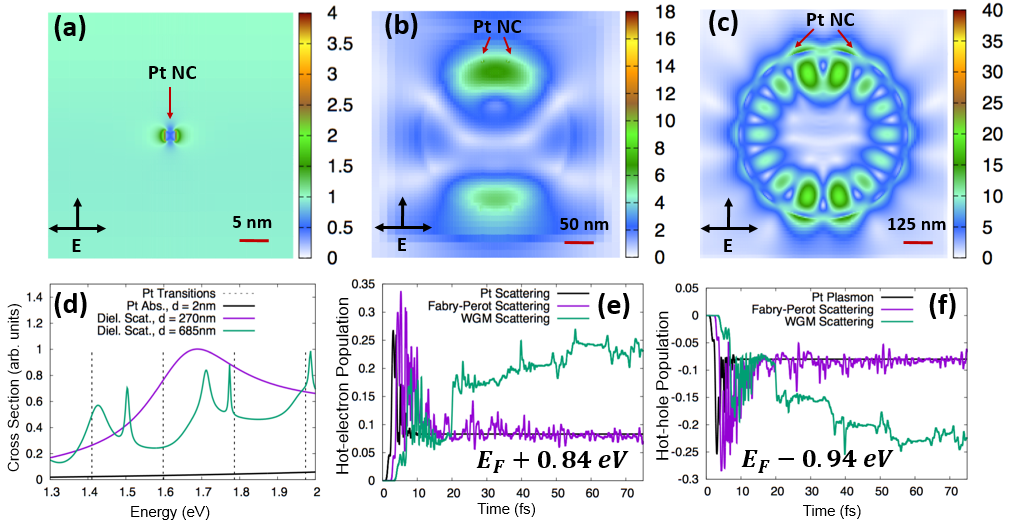
\includegraphics[width=6in]{Pt_AllThree_Revision.png}
\caption{Three regimes for light-matter interactions leading to unique
spatial and temporal shaping of the incident field, and the corresponding
impact on electronic dynamics in a $L=2nm$ PIW Pt nanocube. Plots of the near-field enhancements (${\bf |E|}/{\bf |E_0|}$) are shown of the
Pt NC's extinction maximum ($\lambda=200 nm$, {\bf Panel (a)}), a Fabry-Perot resonance of a d=270nm dielectric nanosphere decorated with Pt NCs
($\lambda = 397 nm$, {\bf Panel (b)}),
and a Whispering Gallery Mode resonance of a d=685 nm dielectric nanosphere decorated with Pt NCs ($\lambda = 493 nm$, {\bf Panel (c)}).
The extinction spectra of these three structures are shown overlaid with the dipole-allowed transitions in the PIW model of the Pt NC, showing partial
overlap between these transitions and the scattering resonances of the $d=685 nm$ dielectric nanosphere ({\bf Panel (d)}).
The change in orbital populations ($^1D_p^p(t)-^1D_P^p(t=0)$) is computed to measure hot-electron and hot-hole generation.
The WGM shows much more efficient generation of hot-electrons ({\bf Panel (e)}) and hot-holes ({\bf Panel(f)}) compared to FP resonance in this case.}
\end{center}
\end{figure}

In contrast to Au, small Pt nanoparticles do not support LSPR at visible wavelengths (see Figure 2 (d)), and consequently, we do not
observe any overlap between an absorption resonance of the $2nm$ Pt nanoparticle and the dipole-allowed 
transitions of our PIW Pt NC model.  We also consider
the same geometries of the dielectric nanospheres as before ($d=270nm$ and $d=685 nm$); the scattering resonances of the former have partial overlap with transitions in the PIW Pt NC model at 1.6 and 1.8 eV, and the resonances of the latter have partial 
overlap with transitions at 1.8, 1.8, and 1.95 eV.  Again, the dielectric scattering resonances provide 
approximately an order of magnitude 
nearfield enhancement in the vicinity of the Pt NC, while the nearfield enhancement provided by the lone 
Pt nanoparticle is much smaller ($|{\bf E}|/|{\bf E_0}| \approx 2$ at $\lambda=200nm$ corresponding to the extinction maximum, see Figure 2 (a), (b), and (c)).
Due to its relatively weak optical interaction, scattering of the Pt nanoparticle does not lead to a large density of hot carriers; small populations
of carriers are created near the Fermi energy (see Figure S2).  These hot carriers can be attributed mostly to direct interaction with the 
incident pulse, which has a peak field strength of $E_0 \approx 614,000,000 \: V/m$, (see SI for more details).
SMA on the $d=270nm$ nanosphere
leads to generation of hot carriers within 1 eV of the Fermi energy with dynamics that persist for moderate (~50 fs) timescales.
The WGMs supported by the $d=685$ dielectric NS show much greater efficiency in creating energetic carriers compared
to the resonances of the $d=270nm$ dielectric NS or the Pt nanoparticle.  For example, WGMs supported by the $d=685nm$ nanosphere are three times
more effective at generating holes in the lowest lying orbital ($E_F - 1.6 eV$) 
and electrons in the highest 
lying orbital ($E_F + 0.84 eV$) in the PIW Pt NC active space as compared to FP resonance of the $d=270nm$ NS (see Figure 2 (e) and (f)).  
The hot carriers driven by WGM also show much more persistent dynamics, and continue to evolve beyond 100 fs (see Figure 2 (e) and (f) and Figure S2).  \textcolor{red}{Fairly rapid fluctuations in the hot-carrier populations 
are observed in both Au and Pt nanoparticles at relatively short times for all three regimes; this presumably results from the
broad distribution of energies in the optical fields that encounter the metal nanoparticles 
at early times combined with
the density of available transition channels.  By contrast, analogous calculations that have a lower density of
transition channels through neglect of excited-state to excited-state transitions show smoother dynamics
(see Figure S4).}
\begin{figure}
\begin{center}
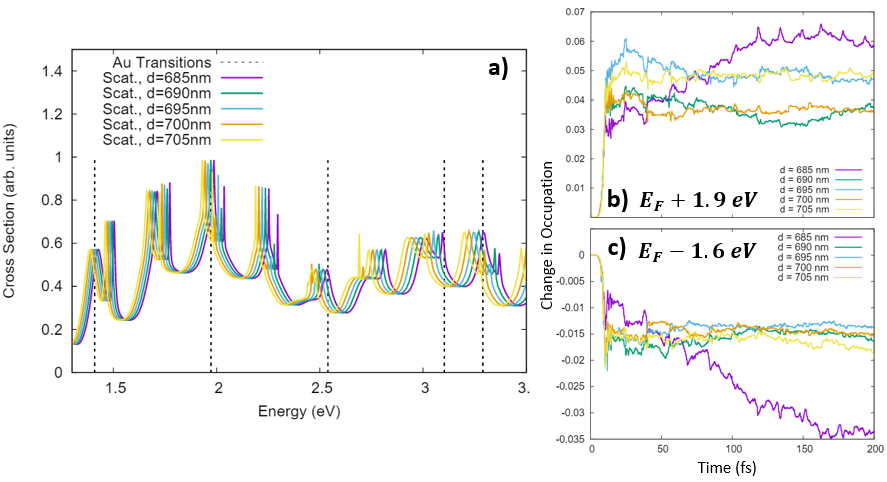
\includegraphics[width=6in]{Au_WGM_Spectrum_and_Trajectories.png}
\caption{Fine-shaping of the spatial and temporal profile of the incident field
through the geometry of the dielectric nanosphere.  Panel {\bf (a)} shows
the scattering spectra of a size progression of dielectric nanospheres that display
predominately Whispering Gallery Mode visible resonances.  The
$685nm$ nanosphere's scattering spectra has the best overlap with the dipole-allowed
transitions in the $L=2nm$ PIW Au NC model, and this structure shows most efficient
generation of hot-electrons in the most energetic orbitals included in our
active space (Panel {\bf (b)}), and more efficiently generation of
hot holes in the lowest energy orbitals included in the PIW Au NC active space (Panel
{\bf (c)}).   }
\end{center}
\end{figure}

To demonstrate the exquisite tunability of the dielectric scattering resonances, and their 
commensurate impact on the electronic dynamics, we consider SMA by a series of 5 different Au-decorated dielectric
nanospheres.  This progression from $d=705 nm$ to $d=685 nm$ brings the dielectric scattering modes progressively 
into resonance with the dipole-allowed transition in the PIW Au NC (see Figure 3 (a)).  We observe efficient hot carrier
generation from SMA in all of these structures, though SMA from the $d=685 nm$ structure leads to most efficient generation
of hot carriers in the highest and lowest energy orbitals in the Au NC active space (see Figure 3(b) and 3(c)), 
most likely owing to the strong overlap between the scattering resonances and the transitions in the Au NC.  

In this work, we have developed a multi-scale theoretical approach that utilizes time-domain electrodynamics to achieve a rigorous description of 
how light is shaped in space and time by interactions with complex nanostructured matter, and bridges this information with a real 
time-dependent configuration interaction singles approach to electronic dynamics.  Importantly, this method goes beyond a perturbative 
inclusion of the electric field and enables us to follow the electronic degrees of freedom subject to strong fields with 
arbitrary time-dependence~\cite{KKS_JCP_2005,GHP_PRA_2010,DPG_PRL_2011}, both of which are characteristic of the nearfields 
resulting from the nanophotonics resonances that were explored in this work.  The explicit inclusion of time-domain fields would 
also enable investigation of time-resolved spectroscopy experiments on similar structures, where the incident fields themselves may be shaped in space and time.  

We have applied this methodology to the study hot carrier generation in novel hybrid nanostructures consisting of large dielectric 
core structures decorated by metal nanoparticles that enable the interplay between scattering resonances in the core 
structure and broadband absorption in the metal nanoparticles, a phenomena known as scattering mediated absorption.  
We have shown that scattering mediated absorption can generate hot carriers while completely circumventing plasmonic resonance.  
This result points to the potential for realizing efficient hot carrier generation and transfer in non-precious metals that are 
earth abundant and cost-effective; \textcolor{red}{future investigations that utilize
more realistic models of the electronic structure will be performed to develop a more detailed
understanding of factors that influence the efficiency of hot-carrier generation in non- or poor plasmonic metals.
Additional developments that focus on a treatment of the optical properties
of the metal that is self-consistent across the electrodynamics and quantum dynamics domains may also be valuable and will be explored.  In principle, the dielectric function may be derived directly from electronic structure calculations of
the metal nanoparticles, and so a self-consistent approach would include deriving the dielectric
function from the same electronic structure model used for the hot-carrier dynamics.  Currently, the electrodynamics
calculations are performed using bulk dielectric data for the metals of interest, though disparities
from bulk behavior have been well documented for particles of this size~\cite{KS_JCP_1983,CTP_3,SKD_Nature_2012,CTP}.
Analogous calculations that utilize size-dependent corrections to
dielectric function in the electrodynamics calculations suggest that the hot-electron dynamics
resulting from SMA may be sensitive to the size-dependent dielectric response of the metal nanoparticles involved,
though the qualitative features of the hot-carrier dynamics reported in this work
are preserved upon inclusion of these corrections (see Figure S5).  The overall similarity 
is likely due to the fact that the scattered field associated with the large dielectric
structure plays the dominant role in driving the dynamics.}   

Our results also reveal that 
unique electronic dynamics can be realized by modulating the frequency and linewidth of the scattering resonances, which 
can be controlled by the size and/or refractive index of the dielectric structure.  In particular, high quality 
factor scattering resonances (e.g. whispering gallery modes) can induce electronic dynamics that persist for hundreds of 
femtoseconds, while plasmonic resonance induces field-driven dynamics on a timescale of ~10 fs.  The ability to 
drive excited-state dynamics of hot carriers through tuning of these resonances may have important implications 
for improving the efficiency and selectivity of photocatalysis via hot carrier transfer, which can be 
severely limited by the rapid decay of energetic carriers resulting from plasmon resonances.

\section{Associated Content}
Additional Figures illustrating hot carrier distributions and dynamics, as well as details of the time-dependent
configuration interaction singles method and the finite-difference time domain simulations are provided in the Supporting 
Information.  This material is available free of charge via the Internet at http://pubs.acs.org

\section{Author Information}
{\bf Corresponding Author}
$^*$ Email: foleyj10@wpunj.edu
\newline
$^{\dagger}$  J.C., N.E., and K.F. contributed equally to this work.
\newline
The authors declare no competing financial interest.

\section{Acknowledgment}
This work was performed, in part, utilizing resources at
the Center for Nanoscale Materials, a US Department of Energy, Office of Science, Office of
Basic Energy Sciences User Facility (contract no. DE-AC02-06CH11357).
JJF Acknowledges the College of Science and Health for startup support.
J.C. and N.E. acknowledge the NSF-GS-LSAMP for support.  K.F. acknowledges the WPU CFR for support.


\bibliography{SMHET} 

\end{document}
   

